\section{Analisi formale della deficienza GAMT}

\begin {frame}
\frametitle {Modellazione formale}
\framesubtitle{Dati preliminari}

\alt<1>{
	\begin{align*}
		Arg + Gly &\xrightleftharpoons{AGAT} Orn + GAA\\
		Met + ATP &\xrightarrow{SAMS} SAM\\
		GAA_{fuori} &\overset{\phantom{\xrightarrow{uptake}}}{\xrightleftharpoons{trasporto}} GAA_{dentro}\\
		GAA_{dentro} + SAM &\xrightarrow{GAMT} Cr + SAH
	\end{align*}
	}
	{
		\begin{align}
		{\color{red}\cancel{\color{black}Arg}} + {\color{red}\cancel{\color{black}Gly}}\nonumber &{\color{red}\cancel{\color{black}\xrightleftharpoons{AGAT}}} {\color{red}\cancel{\color{black}Orn}} + GAA\\
		%Arg + Gly &\xrightleftharpoons{AGAT} Orn + GAA\\
		{\color{gray}Met + ATP} &\xrightarrow{SAMS} SAM\label<1->{sams}\\
		GAA_{fuori} &{\color{red}\overset{\xrightarrow{uptake}}{\cancel{\color{black}\xrightleftharpoons{trasporto}}}} GAA_{dentro}\label<1->{uptake}\\
		GAA_{dentro} + SAM &\xrightarrow{GAMT} Cr + SAH\label<1->{gamt}
		\end{align}
		}


\visible<2>{
	\begin{columns}
		\column{.5\textwidth}
		(\ref{sams}) e (\ref{gamt}) hanno cinetica: $V(A, B) = \frac{\frac{V_{max}}{K_{MA} + [A]} \cdot [B]}{\frac{K_i \cdot K_{MA} + K_{MB} \cdot [A]}{K_{MA} + [A]} + [B]}$
		\column{.5\textwidth}
		(\ref{uptake}) ha cinetica: $V(X_{fuori}, X_{dentro}) = V_{uptake} \cdot ([X]_{fuori} - [X]_{dentro})$
	\end{columns}
	}
\end{frame}

\iffalse

\begin {frame}
\frametitle {Modellazione formale}
\framesubtitle{Modello Bio-PEPA: cinetiche}
\begin{align*}
	sams &= \left [10 \cdot \frac{\frac{v\_sams}{km\_sams\_atp + atp} \cdot met}{\frac{ki\_sams\_sam \cdot km\_sams\_atp + km\_sams\_met \cdot atp}{km\_sams\_atp + atp} + met} \right ]\\
	gamt &= \left [10 \cdot \frac{\frac{v\_gamt}{km\_gamt\_sam + \frac{SAM}{10}} \cdot \frac{GAA\_INT}{10}}{\frac{ki\_gamt\_sah \cdot km\_gamt\_sam + km\_gamt\_gaa\_int \cdot \frac{SAM}{10}}{km\_gamt\_sam + \frac{SAM}{10}} + \frac{GAA\_INT}{10}}\right ]\\
	uptake &= \left [v\_uptake \cdot \frac{GAA\_EXT - GAA\_INT}{10} \right ]
\end{align*}
\end{frame}

\fi

\begin {frame}
\frametitle {Modellazione formale}
\framesubtitle{Modello Bio-PEPA: processi}
\begin{align*}
SAM &= sams \uparrow SAM + gamt \downarrow SAM\\
SAH &= gamt \uparrow SAH\\
GAA\_INT &= uptake \uparrow GAA\_INT + gamt \downarrow GAA\_INT\\
GAA\_EXT &= uptake \downarrow GAA\_EXT\\
CR &= gamt \uparrow CR
\end{align*}
\begin{equation*}
	(SAM \underset{gamt}{\bowtie} SAH \underset{gamt}{\bowtie} GAA\_INT \underset{gamt}{\bowtie} CR)\underset{uptake}{\bowtie} GAA\_EXT
\end{equation*}
\end{frame}

\begin {frame}
\frametitle {Modellazione formale}
\framesubtitle{Modello Bio-PEPA: parametri}
{
\begin{columns}[t]
	\column{.3\textwidth}
	\begin{block}
	{Validazione uptake guanidinoacetato}
	\begin{itemize}
		\item GAA esterno: 10, 25, 50, 100 $\mu M$
		\item Nessun'altra specie chimica
		\item Solo uptake (0.02 $\mu M / min$)
		\invisible{\item SAMS nativa (0.033 $\mu M / min$)}
	\end{itemize}
	\end{block}
	\column{.3\textwidth}
	\begin{block}{Validazione dosaggio creatina}
		\begin{itemize}
			\item GAA esterno: 100 $\mu M$
			\item SAM: 3.5 (valore fisiologico), 10, 50 $\mu M$
			\item GAMT assente (controllo) e circa 0.66 $mg/ml$ (33 $\mu M/min$)
			\item SAMS nativa (0.033 $\mu M / min$)
		\end{itemize}
	\end{block}
	\column{.3\textwidth}
	\begin{block}{Previsione nuovi esperimenti}
		\begin{itemize}
			\item GAA esterno: 50 $\mu M$
			\item SAM: 3.5 $\mu M$
			\item 0.3 $mg/ml $ di GAMT  (15 $\mu M/min$)
			\item SAMS nativa (controllo) e di \emph{E.\ coli} (400 $\mu M/min/mg$):  0.05, 0.1, 0.5, 1, 2.5, 5 $mg$
		\end{itemize}
	\end{block}
\end{columns}
}
\end{frame}

\begin {frame}
\frametitle {Modellazione formale}
\framesubtitle{Modelli PRISM}
\begin{figure}
	\centerline{\resizebox{\paperwidth}{!}{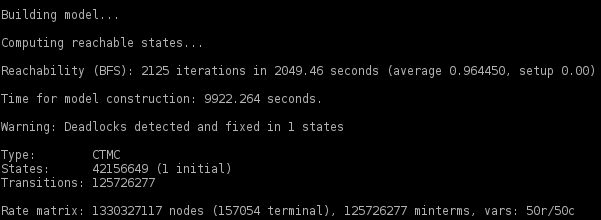
\includegraphics{prism.png}}}
\end{figure}
\end{frame}

\begin {frame}
\frametitle {Analisi simulativa}
\framesubtitle{Uptake}
\begin{figure}
	\center
	\resizebox{!}{0.7\paperheight}{
		\begin{tikzpicture}[spy using outlines={rectangle, magnification=3.0}, connect spies]
		\begin{axis}[axis lines=middle, xmin=0, xmax=60, ymin=0, ymax=70,samples=1000, xtick={0,10,...,60}, xlabel={$t~(min)$}, ylabel={$[GAA*]~(\mu M)$}, legend style={font=\tiny},
		x label style={at={(axis description cs:0.5,-0.1)},anchor=north},
		y label style={at={(axis description cs:-0.1,.5)},rotate=90,anchor=south},
		tick label style={font=\tiny},
		label style={font=\tiny},
		legend pos=outer north east,
		legend entries={$10 \mu M$ GAA*, $25 \mu M$ GAA*, $50 \mu M$ GAA*, $100 \mu M$ GAA*, Sperimentali}]
		
		\addplot[
		ultra thin,
		scatter,forget plot,
		point meta=explicit symbolic,
		scatter/classes={
			gaa10={mark=asterisk,draw=black,mark size=2},
			gaa25={mark=pentagon, draw=black,mark size=2},
			gaa50={mark=diamond, draw=black,mark size=2},
			gaa100={mark=o,draw=black,mark size=2},
			uptakeexp={mark=+,draw=black,mark size=2}}
		]
		file{Dati/001-004/001.txt};
		
		\addplot[
		ultra thin,
		scatter,forget plot,
		point meta=explicit symbolic,
		scatter/classes={
			gaa10={mark=asterisk,draw=black,mark size=2},
			gaa25={mark=pentagon, draw=black,mark size=2},
			gaa50={mark=diamond, draw=black,mark size=2},
			gaa100={mark=o,draw=black,mark size=2},
			uptakeexp={mark=+,draw=black,mark size=2}}
		]
		file{Dati/001-004/002.txt};
		
		
		
		\addplot[
		ultra thin,
		scatter,forget plot,
		point meta=explicit symbolic,
		scatter/classes={
			gaa10={mark=asterisk,draw=black,mark size=2},
			gaa25={mark=pentagon, draw=black,mark size=2},
			gaa50={mark=diamond, draw=black,mark size=2},
			gaa100={mark=o,draw=black,mark size=2},
			uptakeexp={mark=+,draw=black,mark size=2}}
		]
		file{Dati/001-004/003.txt};
		
		\addplot[
		ultra thin,
		scatter,forget plot,
		point meta=explicit symbolic,
		scatter/classes={
			gaa10={mark=asterisk,draw=black,mark size=2},
			gaa25={mark=pentagon, draw=black,mark size=2},
			gaa50={mark=diamond, draw=black,mark size=2},
			gaa100={mark=o,draw=black,mark size=2},
			uptakeexp={mark=+,draw=black,mark size=2}}
		]
		file{Dati/001-004/004.txt};
		
		\addplot[
		ultra thin,
		scatter,
		point meta=explicit symbolic,
		only marks,
		forget plot,
		scatter/classes={
			gaa10={mark=asterisk,draw=black,mark size=2},
			gaa25={mark=pentagon, draw=black,mark size=2},
			gaa50={mark=diamond, draw=black,mark size=2},
			gaa100={mark=o,draw=black,mark size=2},
			uptakeexp={mark=+,draw=black,mark size=2}}
		]
		file{Dati/uptake.txt};
		
		\addlegendimage{mark=asterisk}
		\addlegendimage{mark=pentagon}
		\addlegendimage{mark=diamond}
		\addlegendimage{mark=o}
		\addlegendimage{only marks, mark=+}
		
		
		
		\end{axis}
		\end{tikzpicture}
	}
\end{figure}

\end{frame}

\begin {frame}
\frametitle {Analisi simulativa}
\framesubtitle{Dosaggio}
\begin{columns}
	\column{.5\textwidth}
\begin{figure}
	\center
	\resizebox{\textwidth}{!}{
		\begin{tikzpicture}[spy using outlines={rectangle, magnification=3.0}, connect spies]
		\begin{axis}[axis lines=middle, xmin=0, xmax=300, ymin=0, ymax=85,samples=1000, xtick={0,60,...,300}, xlabel={$t~(min)$}, ylabel={$[Gaa_{int}]~(\mu M)$}, legend style={font=\tiny},
		x label style={at={(axis description cs:0.5,-0.1)},anchor=north},
		y label style={at={(axis description cs:-0.1,.5)},rotate=90,anchor=south},
		tick label style={font=\tiny},
		label style={font=\tiny},
		legend pos=outer north east, mark repeat={10}]
		
		\addplot[
		ultra thin,
		scatter,
		point meta=explicit symbolic,
		scatter/classes={
			sam10={mark=asterisk,draw=black,mark size=2},
			sam50={mark=pentagon, draw=black,mark size=2},
			unload={mark=diamond, draw=black,mark size=2}}
		]
		file{Dati/005-007/005-gaa.txt};
		
		
		
		\addplot[
		ultra thin,
		scatter,
		point meta=explicit symbolic,
		scatter/classes={
			sam10={mark=asterisk,draw=black,mark size=2},
			sam50={mark=pentagon, draw=black,mark size=2},
			unload={mark=diamond, draw=black,mark size=2}}
		]
		file{Dati/005-007/006-gaa.txt};
		
		\addplot[
		ultra thin,
		scatter,
		point meta=explicit symbolic,
		scatter/classes={
			sam10={mark=asterisk,draw=black,mark size=2},
			sam50={mark=pentagon, draw=black,mark size=2},
			unload={mark=diamond, draw=black,mark size=2}}
		]
		file{Dati/005-007/007-gaa.txt};
		
		
		\legend{$10 \mu M$ SAM, $50 \mu M$ SAM, Unloaded};
		
		\coordinate (spypoint) at (axis cs:10,65);
		\coordinate (spyviewer) at (axis cs:100,20);
		\end{axis}
		\spy [height=2.5cm, width=3cm,spy connection path={
			\begin{scope}[on background layer]
			\draw (tikzspyonnode.north east) -- (tikzspyinnode.north east);
			\draw (tikzspyonnode.north west) -- (tikzspyinnode.north west);
			\draw (tikzspyonnode.south west) -- (tikzspyinnode.south west);
			\draw (tikzspyonnode.south east) -- (tikzspyinnode.south east);
			\end{scope}
		}] on (spypoint)
		in node [fill=white] at (spyviewer);
		\end{tikzpicture}
	}
\end{figure}
\column{.5\textwidth}
\begin{figure}
	\center
	\resizebox{\textwidth}{!}{
		\begin{tikzpicture}
		\begin{axis}[axis lines=middle, xmin=0, xmax=120, ymin=0, ymax=60,samples=1000, xtick={0,20,...,120}, xlabel={$t~(min)$}, ylabel={$[Cr]~(\mu M)$}, legend style={font=\tiny},
		x label style={at={(axis description cs:0.5,-0.1)},anchor=north},
		y label style={at={(axis description cs:-0.1,.5)},rotate=90,anchor=south},
		tick label style={font=\tiny},
		label style={font=\tiny},
		legend pos=outer north east, mark repeat={3}]
		
		\addplot[
		ultra thin,
		scatter,
		point meta=explicit symbolic,
		scatter/classes={
			sam10={mark=asterisk,draw=black,mark size=2},
			sam50={mark=pentagon, draw=black,mark size=2},
			unload={mark=diamond, draw=black,mark size=2}}
		]
		file{Dati/005-007/005-cr.txt};
		
		
		
		\addplot[
		ultra thin,
		scatter,
		point meta=explicit symbolic,
		scatter/classes={
			sam10={mark=asterisk,draw=black,mark size=2},
			sam50={mark=pentagon, draw=black,mark size=2},
			unload={mark=diamond, draw=black,mark size=2}}
		]
		file{Dati/005-007/006-cr.txt};
		
		\addplot[
		ultra thin,
		scatter,
		point meta=explicit symbolic,
		scatter/classes={
			sam10={mark=asterisk,draw=black,mark size=2},
			sam50={mark=pentagon, draw=black,mark size=2},
			unload={mark=diamond, draw=black,mark size=2}}
		]
		file{Dati/005-007/007-cr.txt};
		
		
		\legend{$10 \mu M$ SAM, $50 \mu M$ SAM, Unloaded};
		
		\end{axis}
		\end{tikzpicture}
	}
\end{figure}
\end{columns}

\end{frame}

\begin {frame}
\frametitle {Analisi simulativa}
\framesubtitle{Nuovi esperimenti}
\begin{columns}
	\column{.5\textwidth}
\begin{figure}
	\center
	\resizebox{\textwidth}{!}{
		\begin{tikzpicture}[spy using outlines={rectangle, magnification=3.0}, connect spies]
		\begin{axis}[axis lines=middle, xmin=0, xmax=600, ymin=0, ymax=55,samples=1000, xtick={0,60,...,600}, xlabel={$t~(min)$}, ylabel={$[Cr]~(\mu M)$}, legend style={font=\tiny},
		x label style={at={(axis description cs:0.5,-0.1)},anchor=north},
		y label style={at={(axis description cs:-0.1,.5)},rotate=90,anchor=south},
		tick label style={font=\tiny},
		label style={font=\tiny},
		legend pos=outer north east, mark repeat={3}]
		
		\addplot[
		ultra thin,
		scatter,
		point meta=explicit symbolic,
		scatter/classes={
			emat={mark=asterisk,draw=black,mark size=2},
			eco005={mark=pentagon, draw=black,mark size=2},
			eco01={mark=diamond, draw=black,mark size=2},
			eco05={mark=o,draw=black,mark size=2},
			eco1={mark=x, draw=black,mark size=2},
			eco25={mark=square,draw=black,mark size=2},
			eco5={mark=triangle,draw=black,mark size=2}}
		]
		file{Dati/008-014/008-cr.txt};
		
		\addplot[
		ultra thin,
		scatter,
		point meta=explicit symbolic,
		scatter/classes={
			emat={mark=asterisk,draw=black,mark size=2},
			eco005={mark=pentagon, draw=black,mark size=2},
			eco01={mark=diamond, draw=black,mark size=2},
			eco05={mark=o,draw=black,mark size=2},
			eco1={mark=x, draw=black,mark size=2},
			eco25={mark=square,draw=black,mark size=2},
			eco5={mark=triangle,draw=black,mark size=2}}
		]
		file{Dati/008-014/009-cr.txt};
		
		
		
		\addplot[
		ultra thin,
		scatter,
		point meta=explicit symbolic,
		scatter/classes={
			emat={mark=asterisk,draw=black,mark size=2},
			eco005={mark=pentagon, draw=black,mark size=2},
			eco01={mark=diamond, draw=black,mark size=2},
			eco05={mark=o,draw=black,mark size=2},
			eco1={mark=x, draw=black,mark size=2},
			eco25={mark=square,draw=black,mark size=2},
			eco5={mark=triangle,draw=black,mark size=2}}
		]
		file{Dati/008-014/010-cr.txt};
		
		\addplot[
		ultra thin,
		scatter,
		point meta=explicit symbolic,
		scatter/classes={
			emat={mark=asterisk,draw=black,mark size=2},
			eco005={mark=pentagon, draw=black,mark size=2},
			eco01={mark=diamond, draw=black,mark size=2},
			eco05={mark=o,draw=black,mark size=2},
			eco1={mark=x, draw=black,mark size=2},
			eco25={mark=square,draw=black,mark size=2},
			eco5={mark=tria del modellongle,draw=black,mark size=2}}
		]
		file{Dati/008-014/011-cr.txt};
		
		\addplot[
		ultra thin,
		scatter,
		point meta=explicit symbolic,
		scatter/classes={
			emat={mark=asterisk,draw=black,mark size=2},
			eco005={mark=pentagon, draw=black,mark size=2},
			eco01={mark=diamond, draw=black,mark size=2},
			eco05={mark=o,draw=black,mark size=2},
			eco1={mark=x, draw=black,mark size=2},
			eco25={mark=square,draw=black,mark size=2},
			eco5={mark=triangle,draw=black,mark size=2}}
		]
		file{Dati/008-014/012-cr.txt};
		
		\addplot[
		ultra thin,
		scatter,
		point meta=explicit symbolic,
		scatter/classes={
			emat={mark=asterisk,draw=black,mark size=2},
			eco005={mark=pentagon, draw=black,mark size=2},
			eco01={mark=diamond, draw=black,mark size=2},
			eco05={mark=o,draw=black,mark size=2},
			eco1={mark=x, draw=black,mark size=2},
			eco25={mark=square,draw=black,mark size=2},
			eco5={mark=triangle,draw=black,mark size=2}}
		]
		file{Dati/008-014/013-cr.txt};
		
		
		\legend{H. sapiens, $0.05mg$, $0.1mg$, $0.5mg$, $1.0mg$, $2.5mg$};
		
		\coordinate (spypoint) at (axis cs:30,5);
		\coordinate (spyviewer) at (axis cs:120,50);
		\end{axis}
		\spy [height=1.5cm, width=2cm,spy connection path={
			\begin{scope}[on background layer]
			\draw (tikzspyonnode.north east) -- (tikzspyinnode.north east);
			\draw (tikzspyonnode.north west) -- (tikzspyinnode.north west);
			\draw (tikzspyonnode.south west) -- (tikzspyinnode.south west);
			\draw (tikzspyonnode.south east) -- (tikzspyinnode.south east);
			\end{scope}
		}] on (spypoint)
		in node [fill=white] at (spyviewer);
		\end{tikzpicture}
	}
\end{figure}
\column{.5\textwidth}
\begin{figure}
	\center
	\resizebox{\textwidth}{!}{
		\begin{tikzpicture}
		\begin{axis}[axis lines=middle, xmin=0, xmax=600, ymin=0, ymax=27
		,samples=1000, xtick={0,60,...,600}, xlabel={$t~(min)$}, ylabel={$[GAA_{int}]~(\mu M)$}, legend style={font=\tiny},
		x label style={at={(axis description cs:0.5,-0.1)},anchor=north},
		y label style={at={(axis description cs:-0.1,.5)},rotate=90,anchor=south},
		tick label style={font=\tiny},
		label style={font=\tiny},
		legend pos=outer north east,mark repeat={3}]
		
		\addplot[
		ultra thin,
		scatter,
		point meta=explicit symbolic,
		scatter/classes={
			emat={mark=asterisk,draw=black,mark size=2},
			eco005={mark=pentagon, draw=black,mark size=2},
			eco01={mark=diamond, draw=black,mark size=2},
			eco05={mark=o,draw=black,mark size=2},
			eco1={mark=x, draw=black,mark size=2},
			eco25={mark=square,draw=black,mark size=2},
			eco5={mark=triangle,draw=black,mark size=2}}
		]
		file{Dati/008-014/008-gaa_int.txt};
		
		\addplot[
		ultra thin,
		scatter,
		point meta=explicit symbolic,
		scatter/classes={
			emat={mark=asterisk,draw=black,mark size=2},
			eco005={mark=pentagon, draw=black,mark size=2},
			eco01={mark=diamond, draw=black,mark size=2},
			eco05={mark=o,draw=black,mark size=2},
			eco1={mark=x, draw=black,mark size=2},
			eco25={mark=square,draw=black,mark size=2},
			eco5={mark=triangle,draw=black,mark size=2}}
		]
		file{Dati/008-014/009-gaa_int.txt};
		
		\addplot[
		ultra thin,
		scatter,
		point meta=explicit symbolic,
		scatter/classes={
			emat={mark=asterisk,draw=black,mark size=2},
			eco005={mark=pentagon, draw=black,mark size=2},
			eco01={mark=diamond, draw=black,mark size=2},
			eco05={mark=o,draw=black,mark size=2},
			eco1={mark=x, draw=black,mark size=2},
			eco25={mark=square,draw=black,mark size=2},
			eco5={mark=triangle,draw=black,mark size=2}}
		]
		file{Dati/008-014/010-gaa_int.txt};
		
		\addplot[
		ultra thin,
		scatter,
		point meta=explicit symbolic,
		scatter/classes={
			emat={mark=asterisk,draw=black,mark size=2},
			eco005={mark=pentagon, draw=black,mark size=2},
			eco01={mark=diamond, draw=black,mark size=2},
			eco05={mark=o,draw=black,mark size=2},
			eco1={mark=x, draw=black,mark size=2},
			eco25={mark=square,draw=black,mark size=2},
			eco5={mark=triangle,draw=black,mark size=2}}
		]
		file{Dati/008-014/011-gaa_int.txt};
		
		\addplot[
		ultra thin,
		scatter,
		point meta=explicit symbolic,
		scatter/classes={
			emat={mark=asterisk,draw=black,mark size=2},
			eco005={mark=pentagon, draw=black,mark size=2},
			eco01={mark=diamond, draw=black,mark size=2},
			eco05={mark=o,draw=black,mark size=2},
			eco1={mark=x, draw=black,mark size=2},
			eco25={mark=square,draw=black,mark size=2},
			eco5={mark=triangle,draw=black,mark size=2}}
		]
		file{Dati/008-014/012-gaa_int.txt};
		
		\addplot[
		ultra thin,
		scatter,
		point meta=explicit symbolic,
		scatter/classes={
			emat={mark=asterisk,draw=black,mark size=2},
			eco005={mark=pentagon, draw=black,mark size=2},
			eco01={mark=diamond, draw=black,mark size=2},
			eco05={mark=o,draw=black,mark size=2},
			eco1={mark=x, draw=black,mark size=2},
			eco25={mark=square,draw=black,mark size=2},
			eco5={mark=triangle,draw=black,mark size=2}}
		]
		file{Dati/008-014/013-gaa_int.txt};
		
		
		
		\legend{H. sapiens, $0.05mg$, $0.1mg$, $0.5mg$, $1.0mg$, $2.5mg$};
		
		\end{axis}
		\end{tikzpicture}
	}
\end{figure}
\end{columns}

\end{frame}

\begin {frame}
\frametitle {Verifica formale}
\framesubtitle{Nuovi esperimenti}

\centering
\begin{tabular}{|c|c|c|}
	\hline
Propriet\`a & Esito & Tempo impiegato\\
\hline\hline
$\mathbb{P}_{=?} [ \mathcal{F}^{ \leq 600 min} \_SAM\_at\_maximum ]$ & 0.99999 & 67152.519 secondi\\
\hline
$\mathbb{P}_{=?} [ \mathcal{F}^{[600 min,600 min]} \_GAA\_INT\_at\_maximum ]$ & 0 & 65071.259 secondi \\
\hline
$\mathbb{R}_{\{\_UM\_SAM\}=?} [ \mathcal{I}=600 min ]$ & 58.49219 $\mu M$ & 65468.829 secondi \\
\hline
$\mathbb{R}_{\{\_UM\_SAH\}=?} [ \mathcal{I}=600 min ]$ & 34.57216 $\mu M$ & 66046.642 secondi \\
\hline
$\mathbb{R}_{\{\_UM\_GAA\_INT\}=?} [ \mathcal{I}=600 min ]$ & 9.61583 $\mu M$ & 65381.08 secondi \\
\hline
$\mathbb{R}_{\{\_UM\_GAA\_EXT\}=?} [ \mathcal{I}=600 min ]$ & 10.812000 $\mu M$ & 65364.411 secondi \\
\hline
$\mathbb{R}_{\{\_UM\_CR\}=?} [ \mathcal{I}=600 min ]$ & 33.27216 $\mu M$ & 65343.736 secondi \\
\hline
$\mathbb{R}_{\{\_sams\}=?} [ \mathcal{C} \leq 600 min ]$ & 882.566 (simulazione) & N/A \\
\hline
$\mathbb{R}_{\{\_gamt\}=?} [ \mathcal{C} \leq 600 min ]$ & 332.971 (simulazione) & N/A \\
\hline
$\mathbb{R}_{\{\_uptake\}=?} [ \mathcal{C} \leq 600 min ]$ & 392.443 (simulazione) & N/A\\
\hline
$\mathbb{P}_{=?} [\mathcal{F} \mathcal{G} \_SAM \leq 10 \mu M]$ & 0 & 292.23 secondi \\
\hline
\end{tabular}

\end{frame}